\section{Contextual constraints}\label{sec:contextualconstraints}
The grammar of Arc is a \gls{cfg} and only expresses the structure of the language. Further contextual constraints are required to specify if a program is well-formed and meaningfully correct. This section describes Arc's contextual constraints: the scope- and type rules.

\subsection{Scope rules}\label{subsec:scoperules}
The scope rules govern visibility, hiding some parts of a program from others. It also rules where certain things are allowed and others are not.

The Arduino language has static scope, with nested and flat block structures~\cite{cppref}. Blocks are declarable within other blocks (nested), but functions within other functions are not (flat). Arc will have similar scope rules, making compilation more straightforward as source code and target code resemble each other when it comes to scope. Figure~\ref{fig:arcscoperules} shows a graphical model of Arc's scope rules.


\begin{figure}[htb!]
    \centering
    \begin{tikzpicture}[
            double/.style={draw, anchor=text, rectangle split,rectangle split parts=2},
            triple/.style={draw, anchor=text, rectangle split,rectangle split parts=3}
        ]
        \node[state,align=center] at (14,0) {Global scope \\
            \tikz{\node[double, align=center]{Function declaration scope \\
                    \tikz{\node[state, align=center] {block scopes \\
                            \tikz{\node[state, align=center] {block scope}}
                        }
                    }
                    \nodepart{second}Task declaration scope \\
                    \tikz{\node[state, align=center] {block scopes}
                    }}}
        };
    \end{tikzpicture}
    \caption{Diagram of the scope structure of Arc.}
    \label{fig:arcscoperules}
\end{figure}


Arc statements and blocks have nested scoping, while function declarations have flat scope and are not declarable inside a scope. However, one key feature of Arc is its \textit{task} construct, which is not present in Arduino and requires particular focus.


A task declaration is like a function declaration and can not be inside another scope. Additionally, declaring local variables inside the scope of a task declaration is not possible. The Protothreads implementation does not guarantee that the values of local variables are preserved when a thread becomes blocked, making it hard to know if using local variables in a thread will work as the programmer intended.

Another solution to this problem could be to hoist local variable declarations within a task declaration into the global scope. However, this hoisting could make static scope checking difficult. Listing~\ref{lst:hoistclash} shows how the hoisting of a locally declared variable may clash with globally declared variables. While the hoisting issue is not unsolvable, it is clearer to disallow variable declarations within a task declaration. Most importantly, writing an Arc task is entirely declarative - tasks are never called, unlike functions.


\begin{listing}[htb!]
    \begin{minted}[label=Scope clash]{text}
        num a = 1;
        task() {
            num a = 2; // hoist causes a clash here
        }
    \end{minted}
    \caption{Example of hoisting that causes a clash.}
    \label{lst:hoistclash}
\end{listing}


To describe the static scope rules of Arc with operational semantics, we use the environment-store model from Figure~\ref{fig:envstomodel}. The environment-store model describes variables as binding to locations and locations binding to values, while the locations and values are then read with partial functions called \textit{environment} and \textit{store}.


\begin{figure}[htb!]
    \centering
    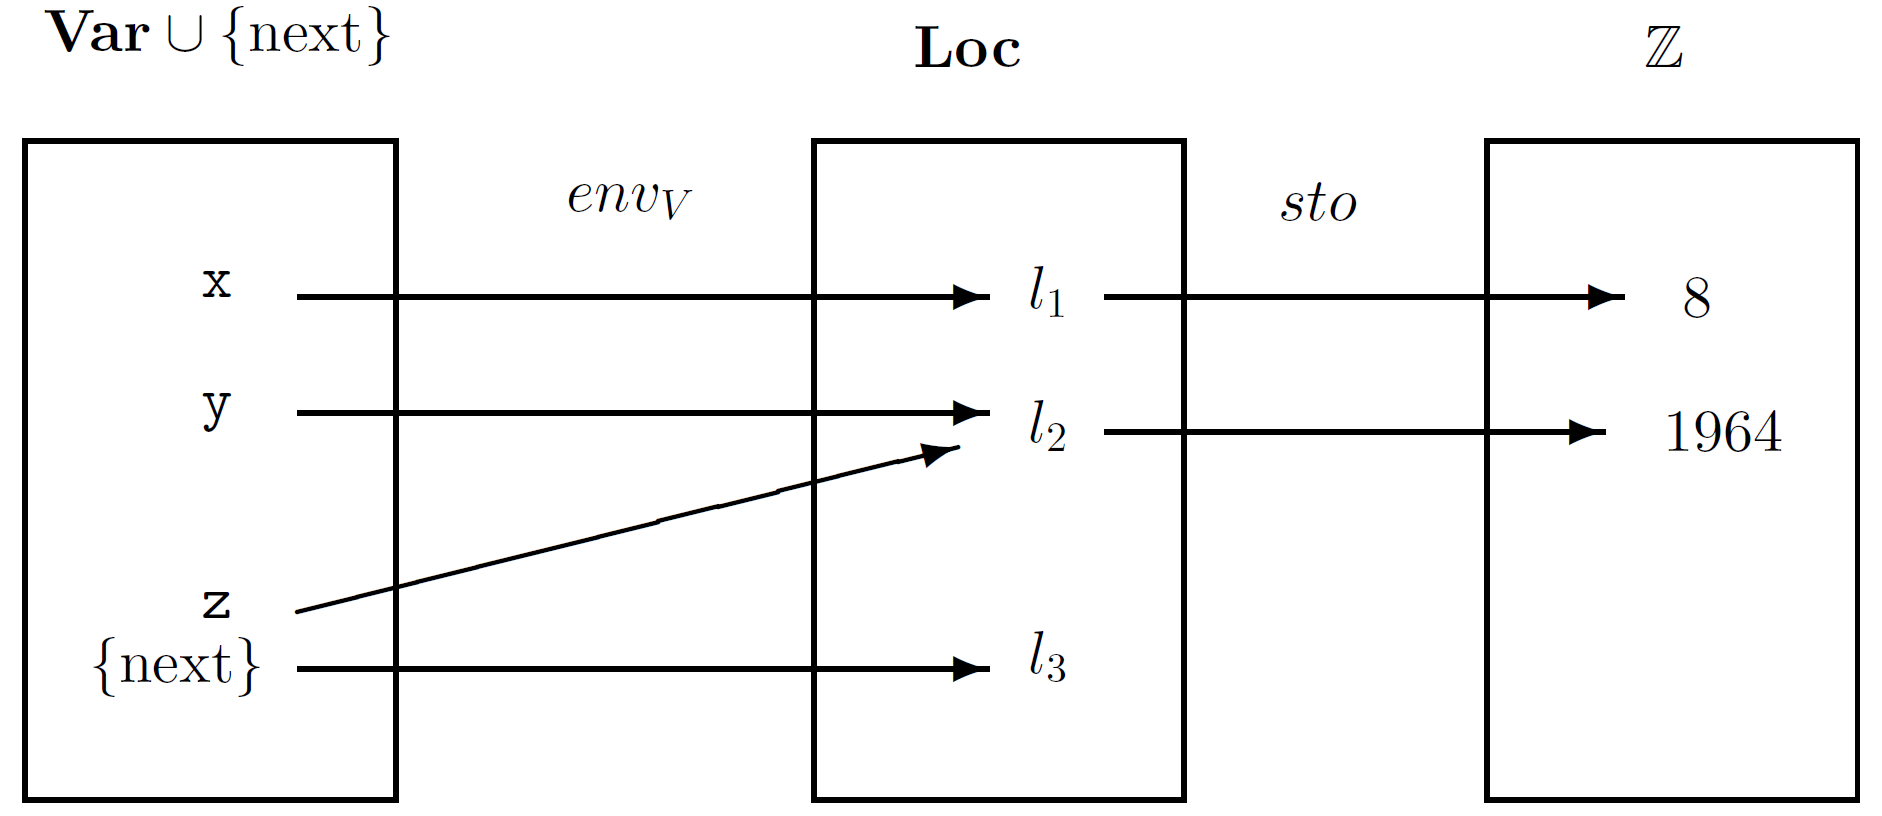
\includegraphics[width=0.8\textwidth]{figures/Environment_Store.png}
    \caption{Example diagram of the environment store model~\cite{Huttel2010}.}
    \label{fig:envstomodel}
\end{figure}


Arc has three environments: the variable environment, the function environment, and the task environment. To describe the semantics of these environments, some function, set, and value names must be defined first. These definitions are presented in Table~\ref{tab:setsandfunctions}, and correspond to rules of Arc's \gls{cfg} described mathematically.

Following the standard of~\cite{Huttel2010}, sets are bolded and begins with a capital letter, while elements are not bolded.


\begin{table}[htb!]
    \centering
    \begin{tabular}{l}
        \toprule
        $\textbf{Val} = \textbf{Num} \cup \textbf{Bool} \cup \textbf{Char} \cup \textbf{Array} \cup \textbf{Pin}\ -$ Values                                            \\
        $\textbf{Pin} = \textbf{PinValues} \times \textbf{Modes}\ -$ Pins are tuples of Arduino pins and modality                                                      \\
        $\textbf{Array} = \mathbb{N} \rightharpoonup \textbf{Val} \setminus \textbf{Pin}\ -$ Arrays map numbers to non-pin values                                      \\
        $\textbf{Par} = \textbf{Types} \times \textbf{Var}\ -$ Set of possible formal parameters                                                                       \\
        $\textbf{Trig} = \{\epsilon, (\text{every} \times \mathbb{N}), (\text{when} \times \textbf{Expr}) \}\ -$ Set of triggers                                       \\
        $v \in \textbf{Val}\ -$ Literal values                                                                                                                         \\
        $x \in \textbf{Var}\ -$ Variable id                                                                                                                            \\
        $f \in \textbf{Fun}\ -$ Function id                                                                                                                            \\
        $t \in \textbf{Types}\ -$ Type names                                                                                                                           \\
        $y \in \textbf{Par}^*\ -$ Formal parameter lists                                                                                                               \\
        $r \in \textbf{Var}^*\ -$ Reference parameter lists                                                                                                            \\
        $S \in \textbf{Stm}\ -$ Statements                                                                                                                             \\
        $l \in \textbf{Loc}\ -$ An arbitrary location in \textbf{Loc}                                                                                                  \\
        next $\ -$ A special 'pointer' holding the value of the next element in \textbf{Loc}                                                                           \\
        new $: \textbf{Loc} \rightarrow \textbf{Loc}\ -$ function to return succesor location                                                                          \\
        \\
        $\textbf{Sto} = \textbf{Loc} \rightharpoonup \textbf{Val}\ -$ Set of stores                                                                                    \\
        $\textbf{Env}_V = \textbf{Var} \cup \{\text{next}\} \rightharpoonup \textbf{Loc}\ -$ Set of variable environments                                              \\
        $\textbf{Env}_F = \textbf{Fun} \rightharpoonup \textbf{Stm} \times \textbf{Par}^* \times \textbf{Env}_V \times \textbf{Env}_F\ -$ Set of function environments \\
        $\textbf{Env}_T = \textbf{Stm} \times \textbf{Var}^* \times \textbf{Trig} \times \textbf{Env}_V \times \textbf{Env}_F\ -$ Set of task environments             \\
        \bottomrule
    \end{tabular}
    \caption{Sets and function definitions.}
    \label{tab:setsandfunctions}
\end{table}


Additionally, we define the notation for updating a given environment $env_V \in \textbf{Env}_V$ we write $env_V[ x \mapsto l]$ to denote the update of $env_V$ given by~\ref{eqn:variableenvironment}


\begin{equation}\label{eqn:variableenvironment}
    env_V[x \mapsto l](y) =
    \begin{cases}
        env_V(y) & y \neq x \\
        l        & y = x
    \end{cases}
\end{equation}


\noindent and $env_F[ f \mapsto (S, y, env_V, env_F)]$ for $env_F$ given by~\ref{eqn:functionenvironment}


\begin{equation}\label{eqn:functionenvironment}
    env_F[f \mapsto (S, y, env_V, env_F)](g) =
    \begin{cases}
        env_F(g)             & g \neq f \\
        (S, y, env_V, env_F) & g = f
    \end{cases}
\end{equation}


\noindent and similarly for a $sto \in \textbf{Sto}$ we write $sto[ l \mapsto v ]$ to indicate the update of $sto$ given by~\ref{eqn:store}


\begin{equation}\label{eqn:store}
    sto[l \mapsto v](l^\prime) =
    \begin{cases}
        sto(l) & l \neq l^\prime \\
        v      & l = l^\prime
    \end{cases}
\end{equation}


With the above definitions of the environment store model and the scope rules, Arc's declarations are described using operational semantics in Table~\ref{tab:arcscoperules}. Because of the static scope rules, the environments are contained within the results of the partial functions for variables and functions. Unlike the variable and function environments, the task environment is not a set of partial functions. This is because unlike function declarations, tasks are not used within other tasks, and does not need to map them.



\begin{table}[htb!]
    \small
    \centering
    \begin{tabular}{ll}
        \toprule
        $[PIN_{DECL}]$  & $\frac
            {\langle env^{\prime\prime}_V, sto[l \mapsto v] \rangle \rightarrow (env^\prime_V, sto^\prime)}
            {\langle \text{\#pin} \ x = (pv, mode), env_V, sto\rangle\rightarrow (env^\prime_V, sto^\prime)}$ \\ [12pt]
                        & where $(pv, mode) \in \textbf{Pin} $                                                \\
                        & and $(pv,mode) \rightarrow v $                                                      \\
                        & and $l = env_V(\text{next})$                                                        \\
                        & and $env^{\prime\prime}_V = env_V[x \mapsto l][\text{next} \mapsto \text{new}(l)] $ \\
        \\

        $[VAR_{DECL}]$  & $\frac
            {\langle env^{\prime\prime}_V, sto[l \mapsto v] \rangle \rightarrow (env^\prime_V, sto^\prime)}
            {\langle t \ x = expr, env_V, sto\rangle\rightarrow (env^\prime_V, sto^\prime)}$                  \\ [12pt]
                        & where $env_V, sto \vdash expr \rightarrow v $                                       \\
                        & and $l = env_V(\text{next})$                                                        \\
                        & and $env^{\prime\prime}_V = env_V[x \mapsto l][\text{next} \mapsto \text{new}(l)] $ \\
        \\

        $[FUNC_{DECL}]$ & $\frac
            {env_V \vdash \langle env_F[f \mapsto \langle S, y, env_V, env_F\rangle] \rangle \rightarrow env^\prime_F}
            {env_V \vdash \langle t \ f (y) \{S \}, env_F \rangle \rightarrow env^\prime_F}$                  \\ [12pt]

        $[TASK_{DECL}]$ & $\frac
            {env_{VF}\vdash \langle env_T[S, r, trig, env_V, envF] \rangle \rightarrow env^\prime_T}
            {env_{VF}\vdash \langle \text{task} \ (r) trig \{S\} \rangle \rightarrow env^\prime_T}$           \\
        \bottomrule
    \end{tabular}
    \caption{Arc's declarations and effects on scope defined with operational semantics.}
    \label{tab:arcscoperules}
\end{table}


To use the declared bindings, we further define their calling and usage. Variables are immutable, and it, therefore, makes sense to have functions use call-by-value for the parameters. Function calls also should not allow recursion, as this makes the runtime memory usage of the Arduino more stable. The semantics for function calls can be seen in Table~\ref{tab:functioncalls}.


\begin{table}[htb!]
    \centering
    \begin{tabular}{ll}
        \toprule
        $FUN_{CALL-1}$ & $\frac
            {env, sto \vdash e_i \Rightarrow e^\prime_i}
            {env, sto \vdash \langle f(\dots, e_i, \dots), env,sto \rangle \rightarrow \langle f(\dots, e^\prime_i, \dots), env, sto \rangle}$ \\ [12pt]
        $FUN_{CALL-2}$ & $\langle f(v_1,\dots,v_i), env, sto \rangle \Rightarrow$                                                              \\
                       & $\qquad \langle \{y_1 = v_1;\dots;y_i = v_i; S\}, (env^\prime_V, env^\prime_F):env, sto \rangle$                      \\ [12pt]

                       & where $env_F(f) = (S, y, env^\prime_V, env^\prime_F)$                                                                 \\
                       & and $env = (env_V, env_F) : env^\prime $                                                                              \\
                       & and $y = y_1,\dots,y_i$                                                                                               \\
        \bottomrule
    \end{tabular}
    \caption{Semantics for function calls.}
    \label{tab:functioncalls}
\end{table}


Tasks are once again unique. Tasks are never called explicitly in Arc code, but the set of all declared tasks serves as the program's entry point. This entry is done through parallel composition and invocation of all declared tasks, of which there must be at least one.

Also of importance is that the parameters of a task describe a mutable reference to a declared variable in $env_V$ that critically cannot be used in another task. This means that task declarations have no formal parameters, only references to actual parameters.

The semantics of the concurrently running tasks are described in Table~\ref{tab:taskinvocation}. The composition of all tasks are created from $env_T$, which is the set of declared tasks, such that $env_T \rightarrow \{T_1 \dots T_n \}$ where $n = |env_T|$.


\begin{table}[htb!]
    \centering
    \begin{tabular}{ll}
        \toprule
        $TASK_{LOOP-1}$ & $\frac
            {(S, env_V, env_F, sto) \Rightarrow (S^\prime, env_V, env_F, sto^\prime)}
            {(\{|\dots T_i \dots|\}, env, sto) \Rightarrow (\{|\dots T_i \dots S^\prime|\}, env, sto^\prime)}$ \\ [12pt]
                        & where $T_i = (S, r, trig, env_V, env_F)$                                             \\ [12pt]
        $TASK_{LOOP-2}$ & $\frac
            {(S, env_V, env_F, sto) \Rightarrow (env_V, env_F, sto^\prime)}
            {(\{|\dots T_i \dots|\}, env, sto) \Rightarrow (\{|\dots T_i \dots|\}, env, sto^\prime)}$          \\ [12pt]
                        & where $T_i = (S, r, trig, env_V, env_F)$                                             \\ [12pt]
        $TASK_{LOOP-3}$ & $\frac
            {(S, env_V, env_F, sto) \Rightarrow (env_V, env_F, sto^\prime)}
            {(\{|\dots T_i \dots S|\}, env, sto) \Rightarrow (\{|\dots T_i \dots|\}, env, sto^\prime)}$        \\
        \bottomrule
    \end{tabular}
    \caption{Semantics for the parallel invocation of tasks as a programs entrypoint.}
    \label{tab:taskinvocation}
\end{table}



\subsection{Type rules}\label{subsec:typerules}
Type rules are another set of contextual constraints. These rules ensure that code fragments do not mistreat types; for example, in static typing, which Arc uses, it should not be possible to assign a number to a variable declared as a boolean~\cite{Sebesta2016}. The valid types in Arc are num, char, bool, and array, as described in section~\ref{sec:inspiration}.

In the type checking semantics the types in the Arc language can be written as:
$T \in \{num, char, bool, N\} N \in \{ 0,\mathbb{N}\}$.


From now on, semantics written mathematically will use T instead of type, if not given a specific type, in semantic type checking. If a specific type is needed, it is written instead of T.

N is not described earlier on what the types are in Arc, as it is not a type that can be declared. N is used for accessing an array; in C++, array access has to have a natural number; this is also implemented in Arc~\cite{cppreferenceDataTypes}.



In declarations and statements type checking, there will be an evaluation to $ok$, which means:

\blockcquote{Huttel2010}{The type of a declaration or a statement will simply be ok; we say that the declaration or statement is well-typed}

In Table~\ref{tab:DeclTypeCheck}, the type checking for variables and functions are written. A specific type function declaration must check if the return type is the same as the declared function type. These declarations are always well-typed as tasks, and void functions do not return values.


\begin{table}[htb!]
    \centering
    \begin{tabular}{ll}
        \toprule
        $[VAR_{DECL}] $  & $\frac{env \vdash expr : T}{env \vdash T \;x = expr : ok}$                            \\  [12pt]
        $[FUNC_{DECL}] $ & $\frac{env \vdash expr : T}{env \vdash T \;f() \{S; \;\text{return} \; expr\}  : ok}$ \\  [12pt]
        $[VOID_{DECL}] $ & $f()\{S\}  : ok$                                                                      \\
        \bottomrule
    \end{tabular}
    \caption{Arc type check for declarations.}
    \label{tab:DeclTypeCheck}
\end{table}


Now that the types have been clarified, it is essential to look at the operations a specific type can do. The first type that will be clarified is num.

In Table~\ref{tab:num-rules}, the operations which the data type num only can do is shown here.


\begin{table}[htb!]
    \centering
    \begin{tabular}{lll}
        \toprule
        $[ADD_{EXPR}] $                         & $\frac
            {env\vdash expr_1: num \quad env\vdash expr_2: num}
            {env\vdash expr_1 \;+\;expr_2: num}$
        \\ [12pt]
        $[SUB_{EXPR}] $                         & $\frac
            {env\vdash expr_1: num \quad env\vdash expr_2: num}
            {env\vdash expr_1 \;-\;expr_2: num}$
        \\ [12pt]
        $[MULT_{EXPR}] $                        & $\frac
            {env\vdash expr_1: num \quad env\vdash expr_2: num}
            {env\vdash expr_1 \;*\;expr_2: num}$
        \\ [12pt]
        $[DIVI_{EXPR}] $                        & $\frac
            {env\vdash expr_1: num \quad env\vdash expr_2: num}
        {env\vdash expr_1 \; / \; expr_2: num}$ & where $expr_2 \neq 0$
        \\ [12pt]
        $[REL_{EXPR}] $                         & $\frac
            {env\vdash expr_1: num \quad env\vdash expr_2: num}
            {env\vdash expr_1 \; OP \; expr_2: Bool}$                                 \\

                                                & where $OP \in \{<, >, \leq, \geq\}$

        \\
        \bottomrule
    \end{tabular}
    \caption{Type rules for num expressions in Arc.}
    \label{tab:num-rules}
\end{table}


The type num is the only type in Arc that can do arithmetic expressions, as it can only do arithmetic expressions on another num type; this can be seen in Table~\ref{tab:num-rules}. The end type of an arithmetic expression is still a num, as it changes the value, not the type.

When comparing, it is also the only type to check if a value is greater or smaller than another num type. When comparing nums, the end type of the expression is a bool, as it is true or false if the num is greater or less than the comparator.


\begin{table}[htb!]
    \centering
    \begin{tabular}{ll}
        \toprule
        $[AND_{EXPR}] $ & $\frac
            {env\vdash expr_1: Bool \quad env\vdash expr_2: Bool}
            {env\vdash expr_1 \;\text{and} \;expr_2: Bool}$
        \\ [12pt]
        $[OR_{EXPR}] $  & $\frac
            {env\vdash expr_1: Bool \quad env\vdash expr_2: Bool}
            {env\vdash expr_1 \;\text{or} \;expr_2: Bool}$
        \\ [12pt]
        $[NOT_{EXPR}] $ & $\frac
            {env\vdash expr_1: Bool}
            {env\vdash \text{not} \; expr_1 : Bool}$
        \\
        \bottomrule
    \end{tabular}
    \caption{Type rules for bool expressions in Arc.}
    \label{tab:bool-rules}
\end{table}


The type bool has three operations that can be seen in Table~\ref{tab:bool-rules}. This means in the And, Or or Not expressions, the expression getting type-checked has to evaluate to bool, and the expressions will then evaluate to another type bool.


\begin{table}[htb!]
    \centering
    \begin{tabular}{ll}
        \toprule
        $[ARRAY_{EXPR}]$      & $ \frac
            {env\vdash expr_1: T \quad env \vdash expr_2 : N}
            {env\vdash expr_1[expr_2] : T}$
        \\ [12pt]
        $[PARENTHESIS_{EXPR}]$ & $ \frac
            {env\vdash expr_1: T}
            {env\vdash (expr_1) : T}$
        \\ [12pt]
        $[EQUAL_{EXPR}] $     & $\frac
            {env\vdash expr_1: T \quad env\vdash expr_2: T}
            {env\vdash expr_1 \;== \;expr_2: Bool}$
        \\ [12pt]
        $[NOTEQUAL_{EXPR}] $  & $\frac
            {env\vdash expr_1: T \quad env\vdash expr_2: T}
            {env\vdash expr_1 \;!= \;expr_2: Bool}$
        \\
        \bottomrule
    \end{tabular}
    \caption{Type rules for other types of expressions in Arc.}
    \label{tab:expr-rules}
\end{table}

The type char does not have any operations that can only be used on that type; therefore, it can only use the expressions that bool and num can do. These type-rules for expressions are written in Table~\ref{tab:expr-rules}. In the array expression, the type N is used to describe the index for the array. The equal and not equal expression evaluates to a bool type, as it can only be true or false.


\begin{table}[htb!]
    \centering
    \begin{tabular}{ll}
        \toprule
        $[COMP_{STMT}] $     & $\frac
            {env \vdash stmt_1 :ok \quad env \vdash stmt_2 :ok}
            {env \vdash stmt_1\;;\;stmt_2: ok}$
        \\ [12pt]
        $[VAR-DECL_{STMT}] $ & $\frac
            {env \vdash expr : T}
            {env \vdash  T \;x = expr: ok}$
        \\ [12pt]
        $[ASSIGN_{STMT}]$    & $\frac
            {env\vdash x: T \quad env \vdash expr : T}
            {env\vdash x = expr: ok}$
        \\ [12pt]
        $[INDEX_{STMT}] $    & $\frac
            {env \vdash x : T \quad env \vdash expr : N \quad env \vdash expr : T}
            {env \vdash x[expr] = expr: ok}$
        \\ [12pt]
        $[BLOCK_{STMT}] $    & $\frac
            {env \vdash stmt :ok}
            {env \vdash \{stmt\}: ok}$
        \\ [12pt]
        $[CALL_{STMT}] $     & $\frac
            {env \vdash f:(x:T \rightarrow ok)\quad env \vdash expr:ok}
            {env \vdash call \;f(expr): ok}$
        \\ [12pt]
        $[RETURN_{STMT}] $   & $\frac
            {env \vdash expr: T}
            {env \vdash \text{return} \;expr: ok}$
        \\ [12pt]
        $[IF_{STMT}] $       & $\frac
            {env \vdash if (expr) : Bool \quad env \vdash stmt_1 :ok \quad env \vdash stmt_2 :ok}
            {env \vdash \text{if} (expr) \;stmt_1 \;\text{else} \;stmt_2: ok}$
        \\ [12pt]
        $[WHILE_{STMT}] $    & $\frac
            {env \vdash  expr : Bool \quad env \vdash stmt :ok}
            {env \vdash \text{while} (expr) \;stmt : ok}$
        \\ [12pt]
        $[FOR_{STMT}] $      & $\frac
            {env \vdash  y : T \quad env \vdash x : T \quad env \vdash block :ok}
            {env \vdash \text{for} (y \; \text{in} \; x) \; block : ok}$
        \\
        \bottomrule
    \end{tabular}
    \caption{Arc type check statements.}
    \label{tab:StatementTypeCheck}
\end{table}


The type checking for statements in Arc can be seen in Table~\ref{tab:StatementTypeCheck}. As explained before, type-checking statements give the same output as the declarations in OK, which means well-typed. A variable can be declared in scope; therefore, it has the same type-check rules as in variable declaration, as shown in Table~\ref{tab:DeclTypeCheck}. Return uses an expression that evaluates to a type T; this type is the same as the type of the function with which it is declared.